% Generated by pysimcount.pfchilds -- do not edit; regenerate instead.
% figure: main-total-suzuki-orders -- Suzuki formulas of each order, total gates vs n (layout of Childs et al. 2018 Fig. 3 right)
% source: ../np-main/aggregate.json + ../np-main-n9/seed{seed}, ../np-main-n11/seed{seed} (seeds [1, 2, 3, 4, 5, 6, 7, 8, 9, 10]); run commits: 01d3c275ceae2840002bd1aaea68f59b987c4975, e42ff29056ad9ea7fc7c9899fab334903e42e3e3
% metric=total kind=xyz merged (cz, simcount template)
% measured n: mean over seeds of the run's totals; bars min..max over seeds
% r from per-seed power-law fits (n = 5--11), mean count over seeds; r = ceil(a n^b); point=seed-mean; bars = min..max of per-seed fits
% per-step counts exactly affine in n (checked on n = [10, 20, 40], direct build at n = [100])
% shown: suzuki4, suzuki6, suzuki8
% removed (see main-total-suzuki-orders-ranking.md): lie-trotter, suzuki2
% figure made at git_commit=e5d9ee696f892e28aced765585653760f8a427c4 git_dirty=False
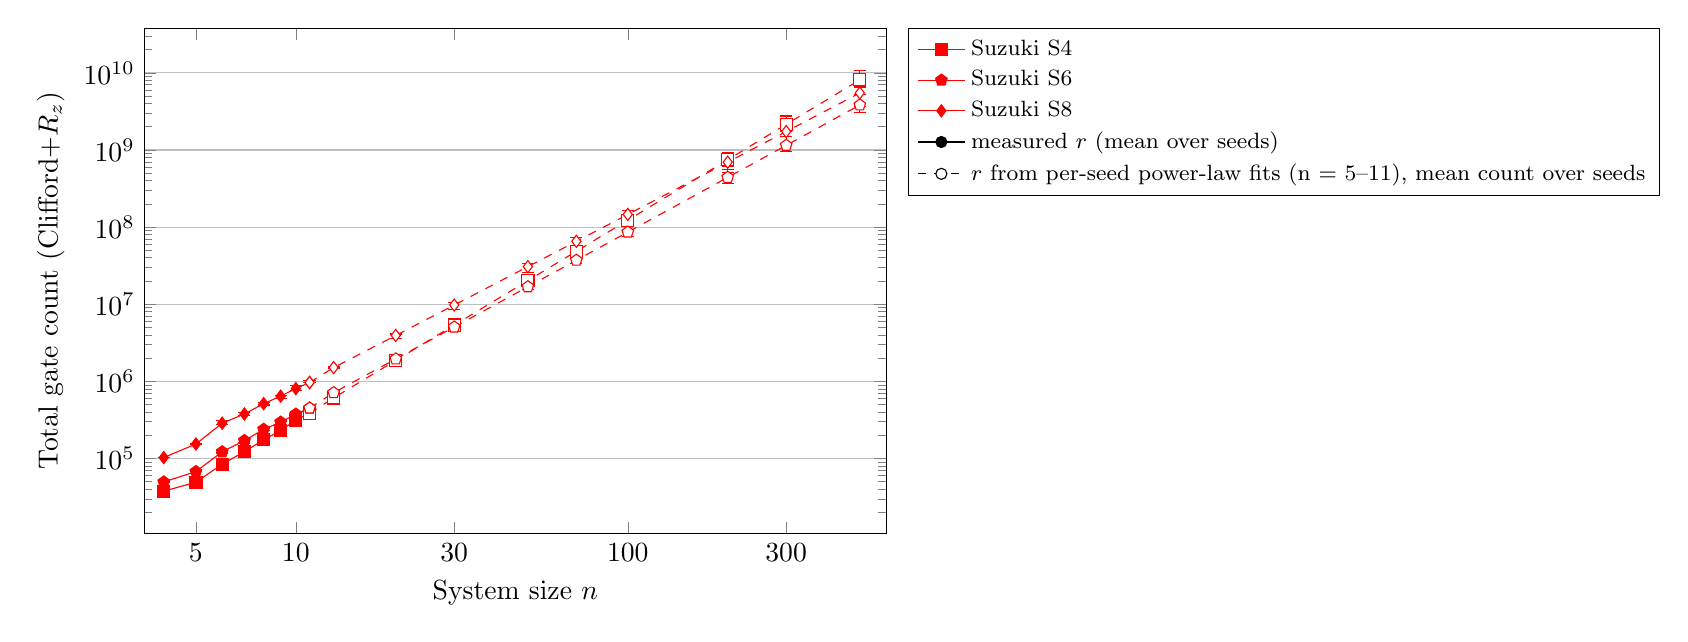
\begin{tikzpicture}
  \begin{loglogaxis}[
    width=11cm, height=8cm,
    xlabel={System size $n$},
    ylabel={Total gate count (Clifford+$R_z$)},
    xtick={5,10,30,100,300}, xticklabels={5,10,30,100,300},
    xmin=3.5, xmax=600,
    ymajorgrids=true,
    legend pos=outer north east,
    legend cell align=left,
    legend style={font=\footnotesize},
  ]
    % suzuki4: measured n, mean over seeds, bars min..max over seeds
    \addplot[red, solid, mark=square*, mark size=2.2pt, mark options={solid, fill=red}, error bars/.cd, y dir=both, y explicit, error bar style={solid}] coordinates {
      (4,37651.2) += (0,508.8) -= (0,339.2)
      (5,49184) += (0,1696) -= (0,1484)
      (6,84333.6) += (0,5978.4) -= (0,4197.6)
      (7,122578) += (0,9497.6) -= (0,8310.4)
      (8,174349) += (0,7123.2) -= (0,6444.8)
      (9,229914) += (0,10494) -= (0,12402)
      (10,315032) += (0,24168) -= (0,11872)
      (11,384780) += (0,16324) -= (0,9328)
    };
    \addlegendentry{Suzuki S4}
    % suzuki4: extrapolated, r = ceil(3.65267 n^1.59931), per step = 212 n + 0; bars min..max of per-seed fits
    \addplot[red, dashed, mark=square*, mark size=2.2pt, mark options={solid, fill=white}, forget plot, error bars/.cd, y dir=both, y explicit, error bar style={solid}] coordinates {
      (11,384780)
      (13,609903) += (0,26733.2) -= (0,20118.8)
      (20,1.86772e+06) += (0,137800) -= (0,103880)
      (30,5.3583e+06) += (0,550140) -= (0,410220)
      (50,2.02333e+07) += (0,2.86412e+06) -= (0,2.07548e+06)
      (70,4.85565e+07) += (0,8.13232e+06) -= (0,5.80244e+06)
      (100,1.22856e+08) += (0,2.39963e+07) -= (0,1.68773e+07)
      (200,7.46656e+08) += (0,1.8712e+08) -= (0,1.27955e+08)
      (300,2.14644e+09) += (0,6.08964e+08) -= (0,4.09718e+08)
      (500,8.12156e+09) += (0,2.64878e+09) -= (0,1.74725e+09)
    };
    % suzuki6: measured n, mean over seeds, bars min..max over seeds
    \addplot[red, solid, mark=pentagon*, mark size=2.2pt, mark options={solid, fill=red}, error bars/.cd, y dir=both, y explicit, error bar style={solid}] coordinates {
      (4,49536) += (0,0) -= (0,0)
      (5,67596) += (0,4644) -= (0,516)
      (6,121982) += (0,8049.6) -= (0,4334.4)
      (7,170486) += (0,10113.6) -= (0,11558.4)
      (8,238598) += (0,9081.6) -= (0,7430.4)
      (9,295358) += (0,11145.6) -= (0,16718.4)
      (10,375648) += (0,26832) -= (0,14448)
      (11,449539) += (0,15892.8) -= (0,6811.2)
    };
    \addlegendentry{Suzuki S6}
    % suzuki6: extrapolated, r = ceil(1.63295 n^1.35284), per step = 1032 n + 0; bars min..max of per-seed fits
    \addplot[red, dashed, mark=pentagon*, mark size=2.2pt, mark options={solid, fill=white}, forget plot, error bars/.cd, y dir=both, y explicit, error bar style={solid}] coordinates {
      (11,449539)
      (13,711048) += (0,40248) -= (0,13416)
      (20,1.95048e+06) += (0,154800) -= (0,72240)
      (30,5.05577e+06) += (0,578952) -= (0,287928)
      (50,1.68216e+07) += (0,2.6832e+06) -= (0,1.4448e+06)
      (70,3.71314e+07) += (0,7.00728e+06) -= (0,3.82872e+06)
      (100,8.60482e+07) += (0,1.89062e+07) -= (0,1.04026e+07)
      (200,4.40808e+08) += (0,1.24521e+08) -= (0,6.86693e+07)
      (300,1.14685e+09) += (0,3.66783e+08) -= (0,2.01642e+08)
      (500,3.82702e+09) += (0,1.40832e+09) -= (0,7.67653e+08)
    };
    % suzuki8: measured n, mean over seeds, bars min..max over seeds
    \addplot[red, solid, mark=diamond*, mark size=2.2pt, mark options={solid, fill=red}, error bars/.cd, y dir=both, y explicit, error bar style={solid}] coordinates {
      (4,102640) += (0,0) -= (0,0)
      (5,153960) += (0,0) -= (0,0)
      (6,286366) += (0,21554.4) -= (0,9237.6)
      (7,377202) += (0,17962) -= (0,17962)
      (8,513200) += (0,20528) -= (0,20528)
      (9,642013) += (0,4618.8) -= (0,41569.2)
      (10,805724) += (0,66716) -= (0,35924)
      (11,965329) += (0,50806.8) -= (0,5645.2)
    };
    \addlegendentry{Suzuki S8}
    % suzuki8: extrapolated, r = ceil(0.896539 n^1.24879), per step = 5132 n + 0; bars min..max of per-seed fits
    \addplot[red, dashed, mark=diamond*, mark size=2.2pt, mark options={solid, fill=white}, forget plot, error bars/.cd, y dir=both, y explicit, error bar style={solid}] coordinates {
      (11,965329)
      (13,1.50778e+06) += (0,26686.4) -= (0,40029.6)
      (20,3.93111e+06) += (0,174488) -= (0,338712)
      (30,9.74567e+06) += (0,723612) -= (0,1.12391e+06)
      (50,3.06894e+07) += (0,2.92524e+06) -= (0,5.02936e+06)
      (70,6.52739e+07) += (0,7.29257e+06) -= (0,1.21064e+07)
      (100,1.45851e+08) += (0,1.83726e+07) -= (0,3.14078e+07)
      (200,6.94462e+08) += (0,1.09209e+08) -= (0,1.86394e+08)
      (300,1.7322e+09) += (0,3.04687e+08) -= (0,5.1746e+08)
      (500,5.48149e+09) += (0,1.0926e+09) -= (0,1.83264e+09)
    };
    \addlegendimage{black, solid, mark=*, mark options={solid, fill=black}}
    \addlegendentry{measured $r$ (mean over seeds)}
    \addlegendimage{black, dashed, mark=*, mark options={solid, fill=white}}
    \addlegendentry{$r$ from per-seed power-law fits (n = 5--11), mean count over seeds}
  \end{loglogaxis}
\end{tikzpicture}
